\subsection{Introduction}
The core concept of the application is to provide to citizens of any city a reliable and fast way to report traffic violations they see on streets, trying to improve their awareness about the topic and addressing a social problem that could potentially harm the viability of the city or cause problems to people with disability. To achieve this goal, SafeStreets behaves as an intermediary between the citizens, who have the responsibility of reporting the violations, and the authorities, who can access the report and take care of them. The system allows an asynchronous interaction between parts, avoiding time loss for both the actors.

The municipalities can also have various benefits too when registered to the system, because SafeStreets provide them a way to integrate their data about violations with the ones stored in SafeStreets' databases, calculating then the most unsafe areas and providing suggestions about possible interventions to improve them.

\subsection{Class diagram}

The following class diagrams shows the model of the application domain and its main actors and entities. Note that this class diagram is really high-level, its main purpose it's only to display the defined entities involved in the system, their principal attributes and the relations between them.

\begin{figure}[H]
	\centering
	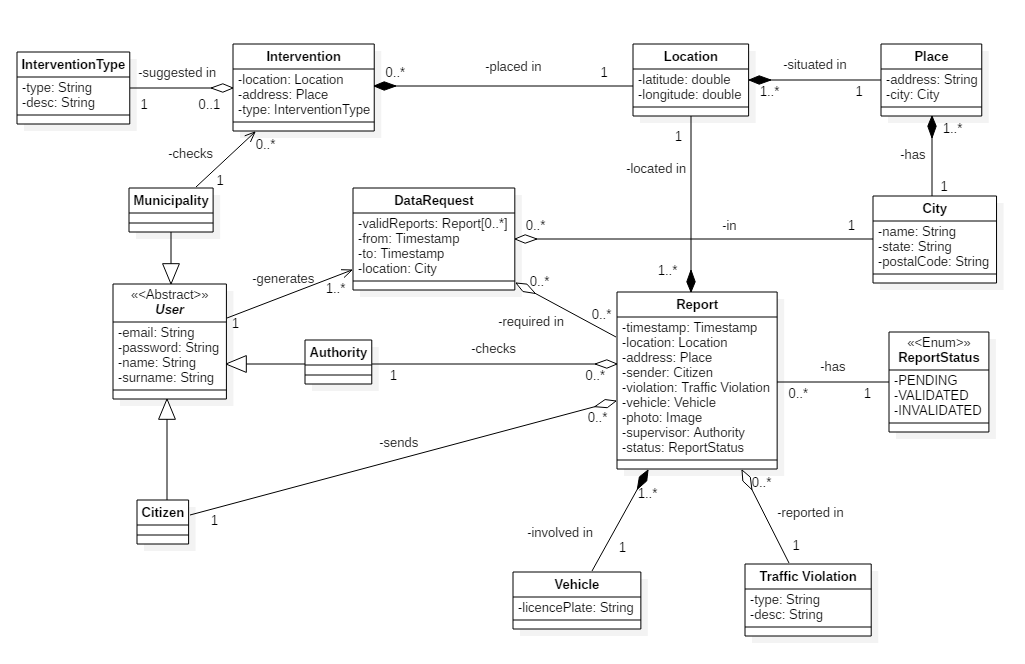
\includegraphics[width=\textwidth]{UML/ClassDiagram}
	\caption{Class diagram}
\end{figure}

User abstract class represents the common structure and attributes shared between all types of accounts that reflect the role of the customers of the system. Citizens' main role is to generate reports to populate the databases of violations, while the authorities can check these reports and update their status from pending (default initial status) to validated or invalidated, based on the fact if the violation has been certified or not. Municipality accounts instead can visualize the list of interventions to improve the situation of detected unsafe areas and also rate the suggestions to give a feedback to the system. All account types can submit data requests for visualizing aggregated information relevant to them, but only authorities can visualize single reports (actually a citizen can visualize single reports too, but only the ones made by himself).

Another important aspect to underline is that Municipalities and Authorities have also a city attribute, that identify the city on which they have jurisdiction. This allow the system to provide them respectively a list of  interventions and reports that are situated in their area of interest. 

Report entity could be considered central in the entire system because it contains various references to many other entities of the model and its essential to achieve the goals of the application. Reports have attributes that specify their type, the date and hour of the violation, and their actual status. Other fields are references to other class objects, like the vehicle involved, the location of the violation, the citizen who submits the report and the authority who has supervised its certification. It's important to note that vehicle and location entities have a strict composition relation with the report entities, this means that if no more reports with that vehicle or location are stored in the system, also the vehicle and location entities are eliminated from the system.

Lastly, the location of a violation or intervention is handled by the Location-Place-City correlated entities. The separation of this entities through composition allows a higher level of granularity and maintainability. Composition is used to emphasize the fact that if no more places of a city are stored in the database, the city is also deleted from it, same thing for places if no more location coordinates of the place are needed.

\subsection{State diagrams}

Next section provides multiple state diagrams, useful to better understand the main actions that the different customers can perform with the application.

\subsubsection{Generate report (citizens)}

\begin{figure}[H]
	\centering
	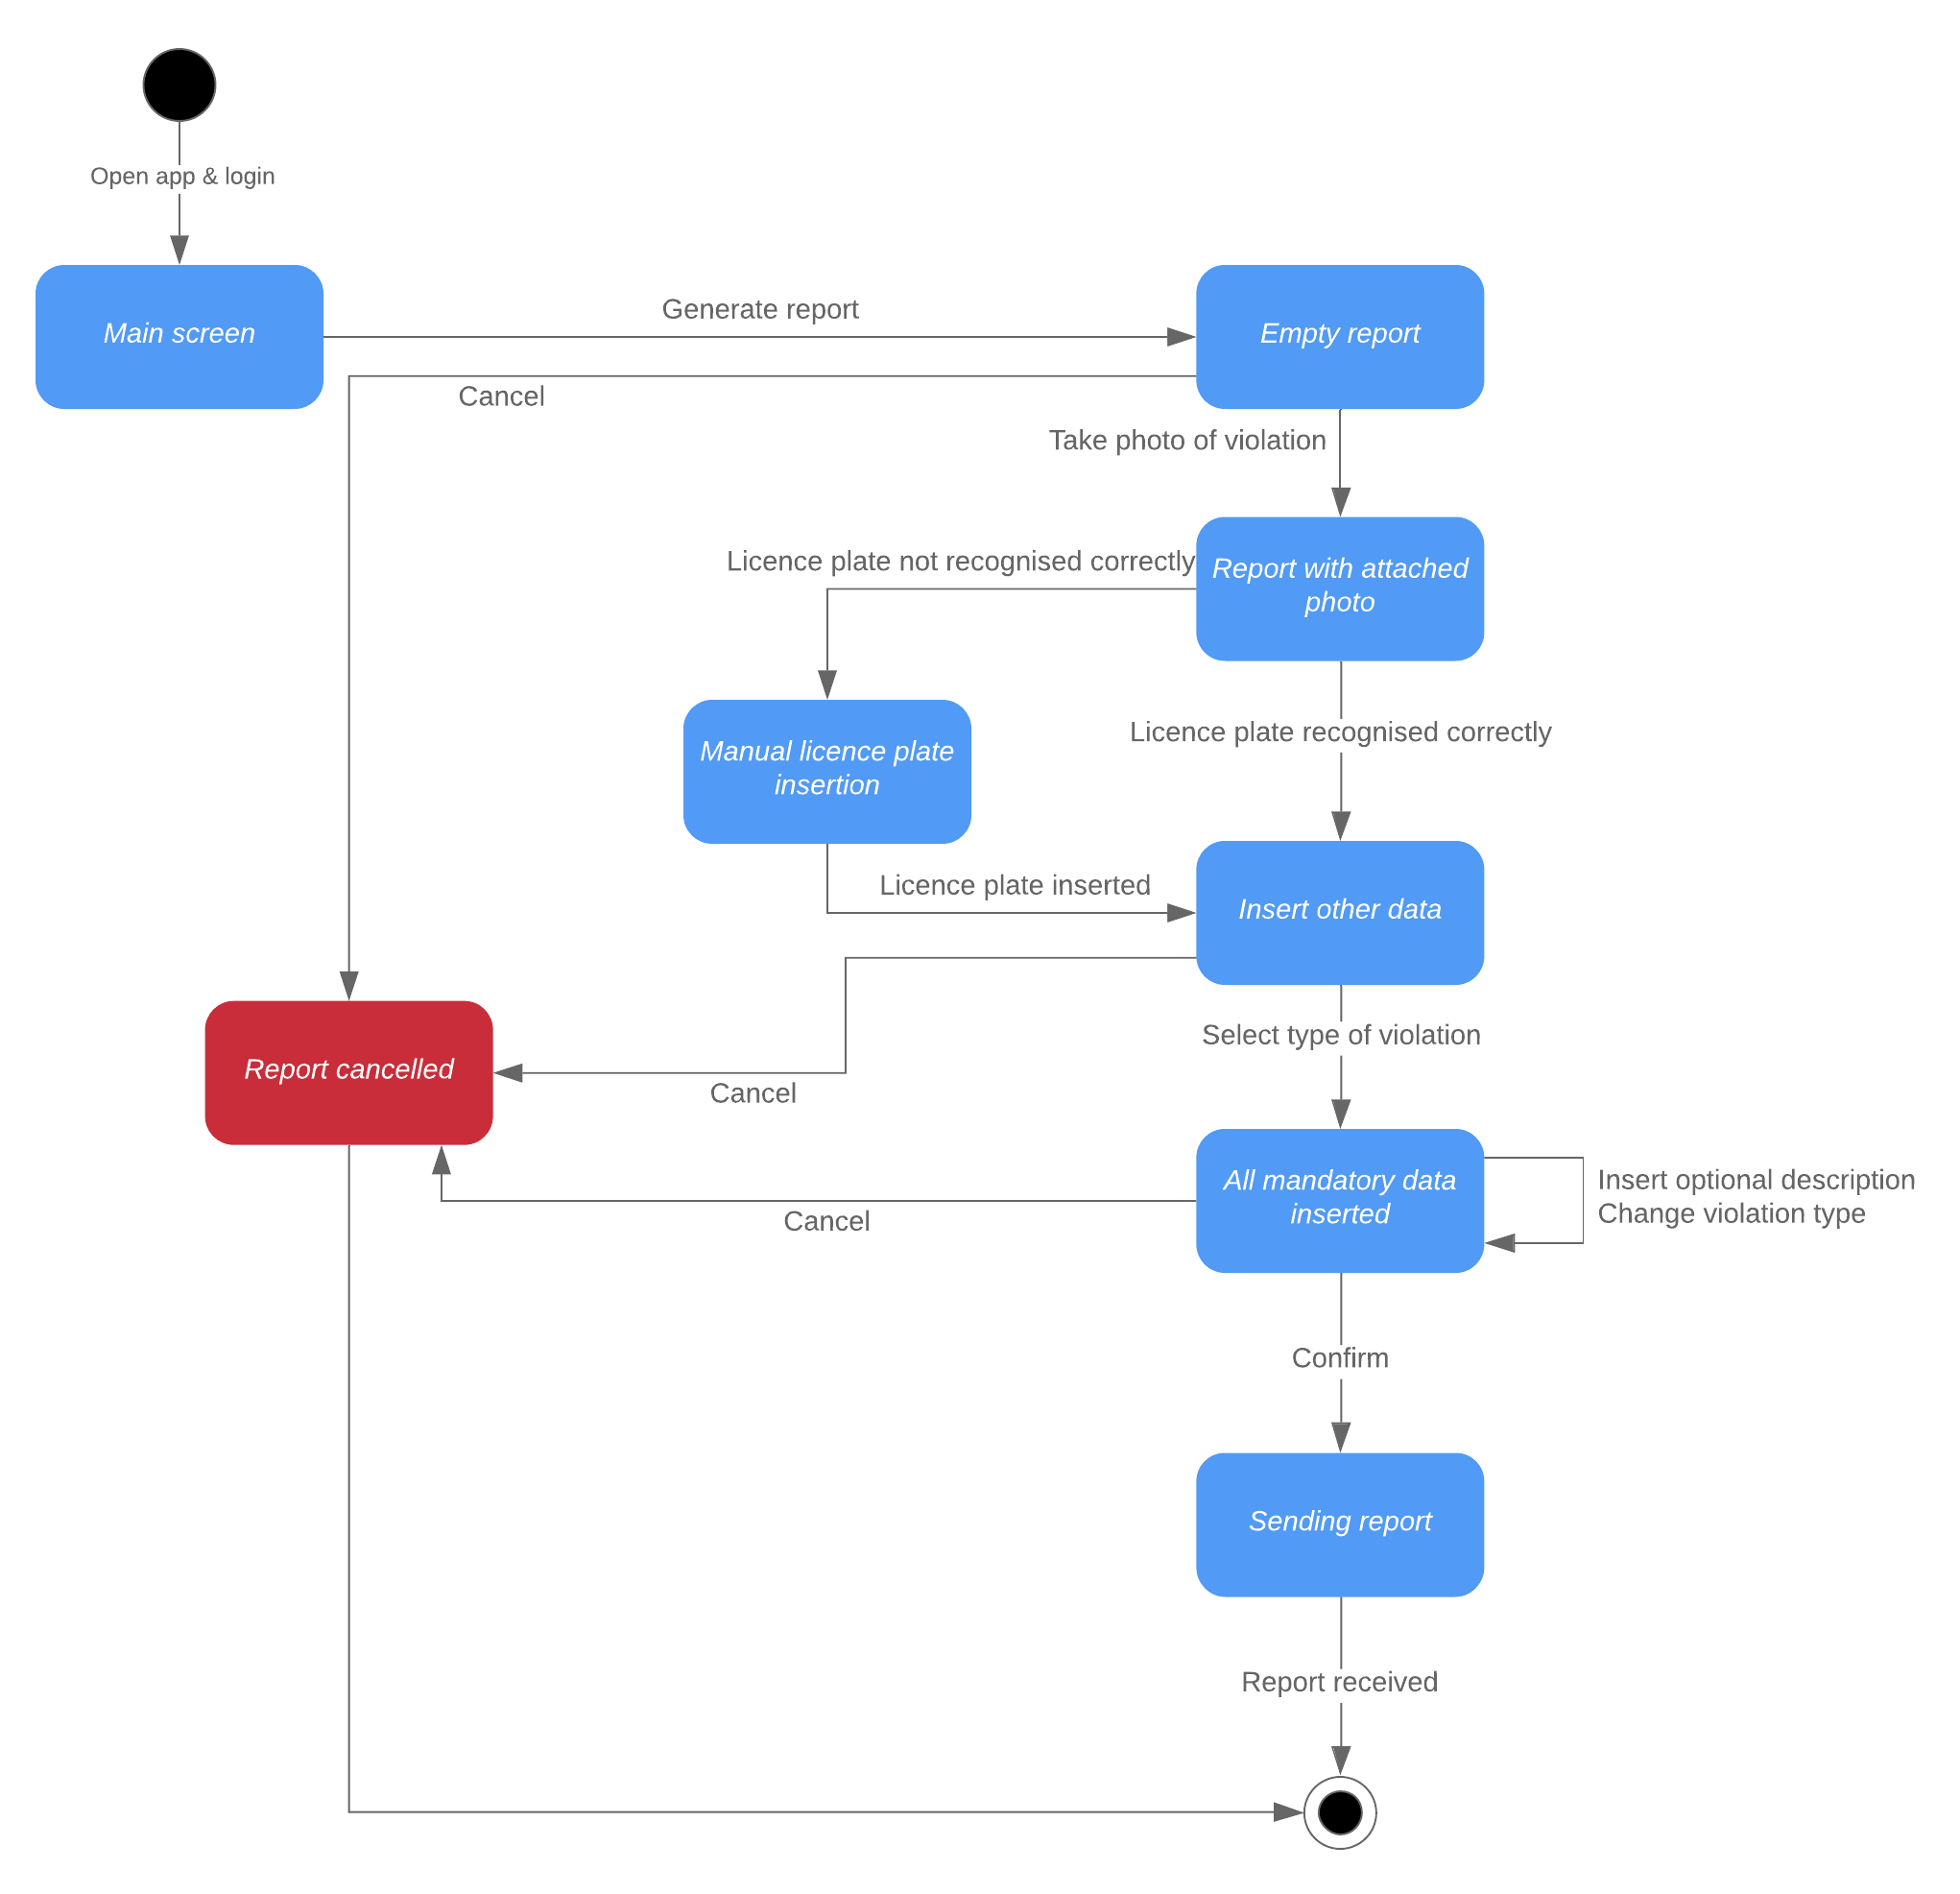
\includegraphics[width=\textwidth]{UML/ReportStateDiagram}
	\caption{Generate report state diagram}
\end{figure}

This state diagram specify all the operations needed to complete and submit a report. After selecting the "generate report" tab, the citizen is asked to take at least one photo of the violation, with the license plate of the transgressor's vehicle clearly visible in the first one. After confirmation, the first photo of the violation is uploaded to SafeStreets servers and used in the OCR service to recognize automatically the license plate. The result is then sent back to the user, that needs to confirm if the license plate has been recognized correctly, if not the user can insert it manually. After that, the citizen needs to select the violation type and check also that location field has been correctly populated by the GPS. If detected location is wrong, user can click a button to try again to get the correct location from the GPS. The description field is completely optional and not required to confirm and submit the report.

\subsubsection{Reports validation (authorities)}

\begin{figure}[H]
	\centering
	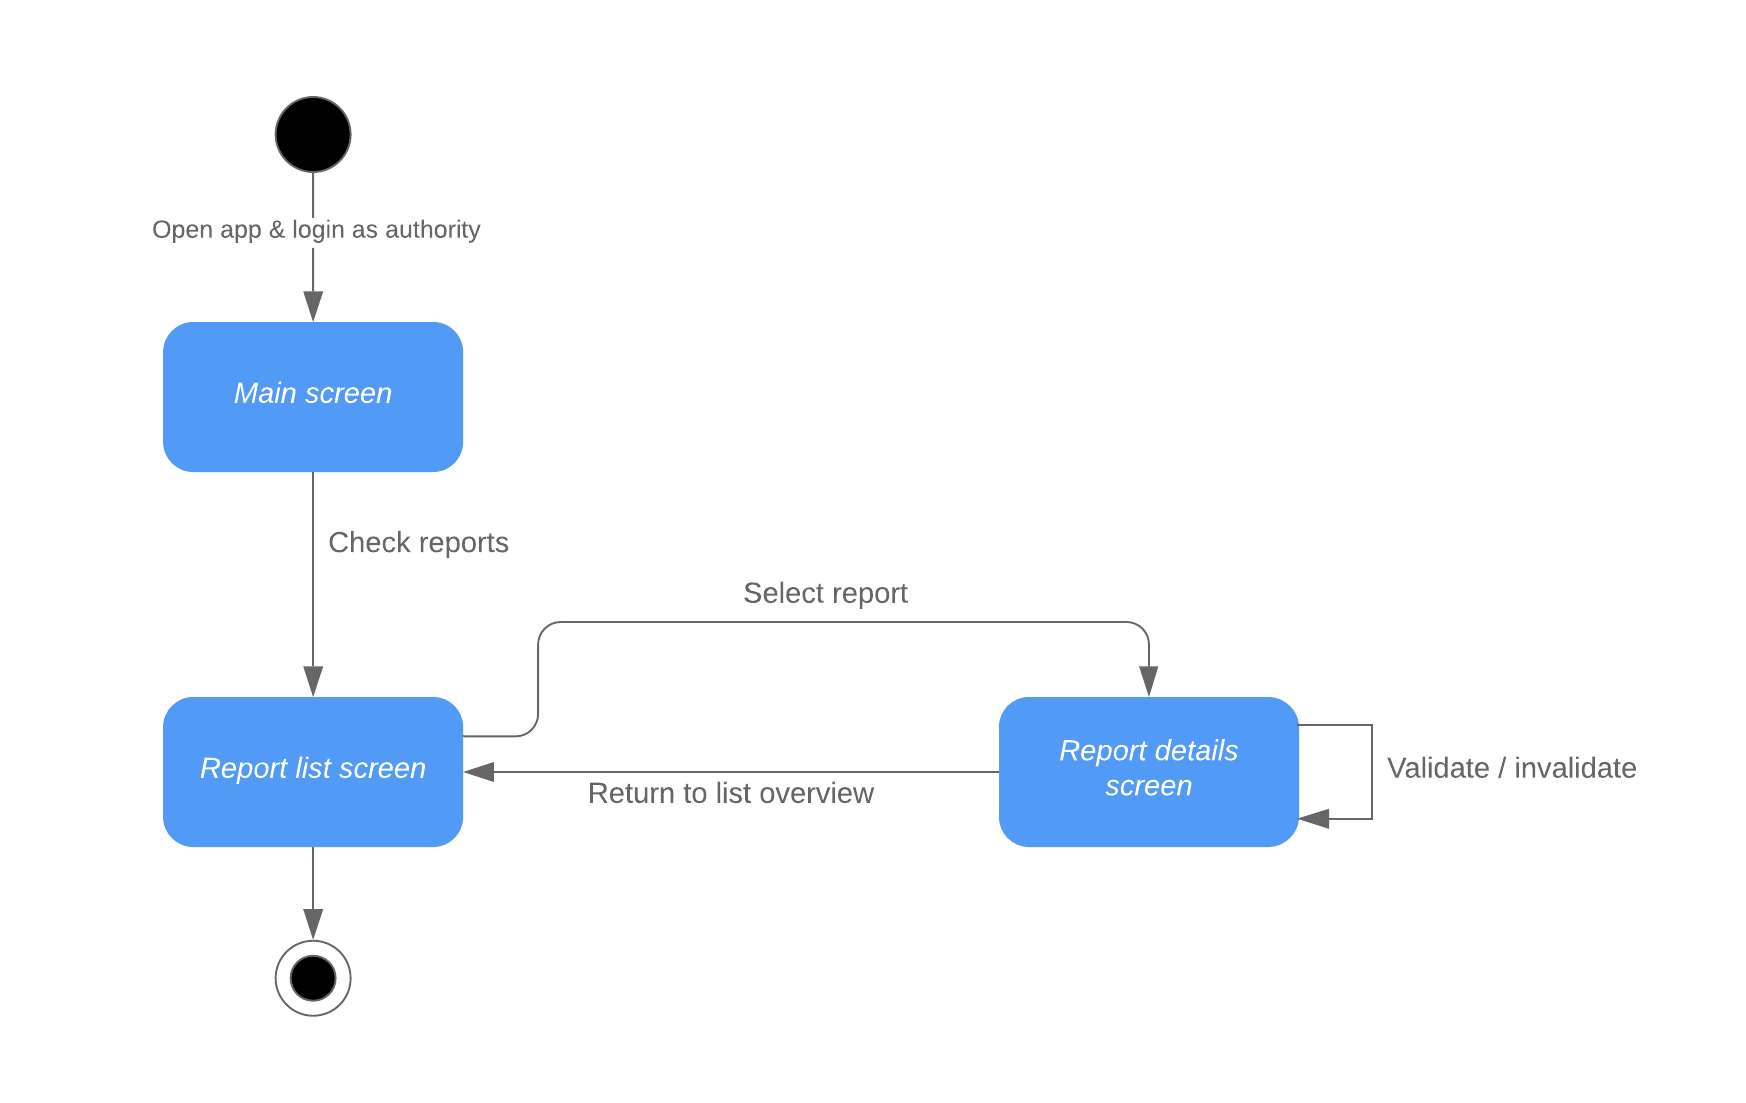
\includegraphics[width=\textwidth]{UML/ReportValidationStateDiagram}
	\caption{Reports validation state diagram}
\end{figure}

This diagram instead focuses on the report supervision performed by the authorities. In appropriate report section, an authority can visualize the whole list of violations occurred in their area of competence and visualize a report at a time to validate or invalidate them. Every time a report is validated or invalidated, the citizen who submitted the report is notified on SafeStreets app about the status change.

\subsubsection{Suggestions evaluation (municipality)}

\begin{figure}[H]
	\centering
	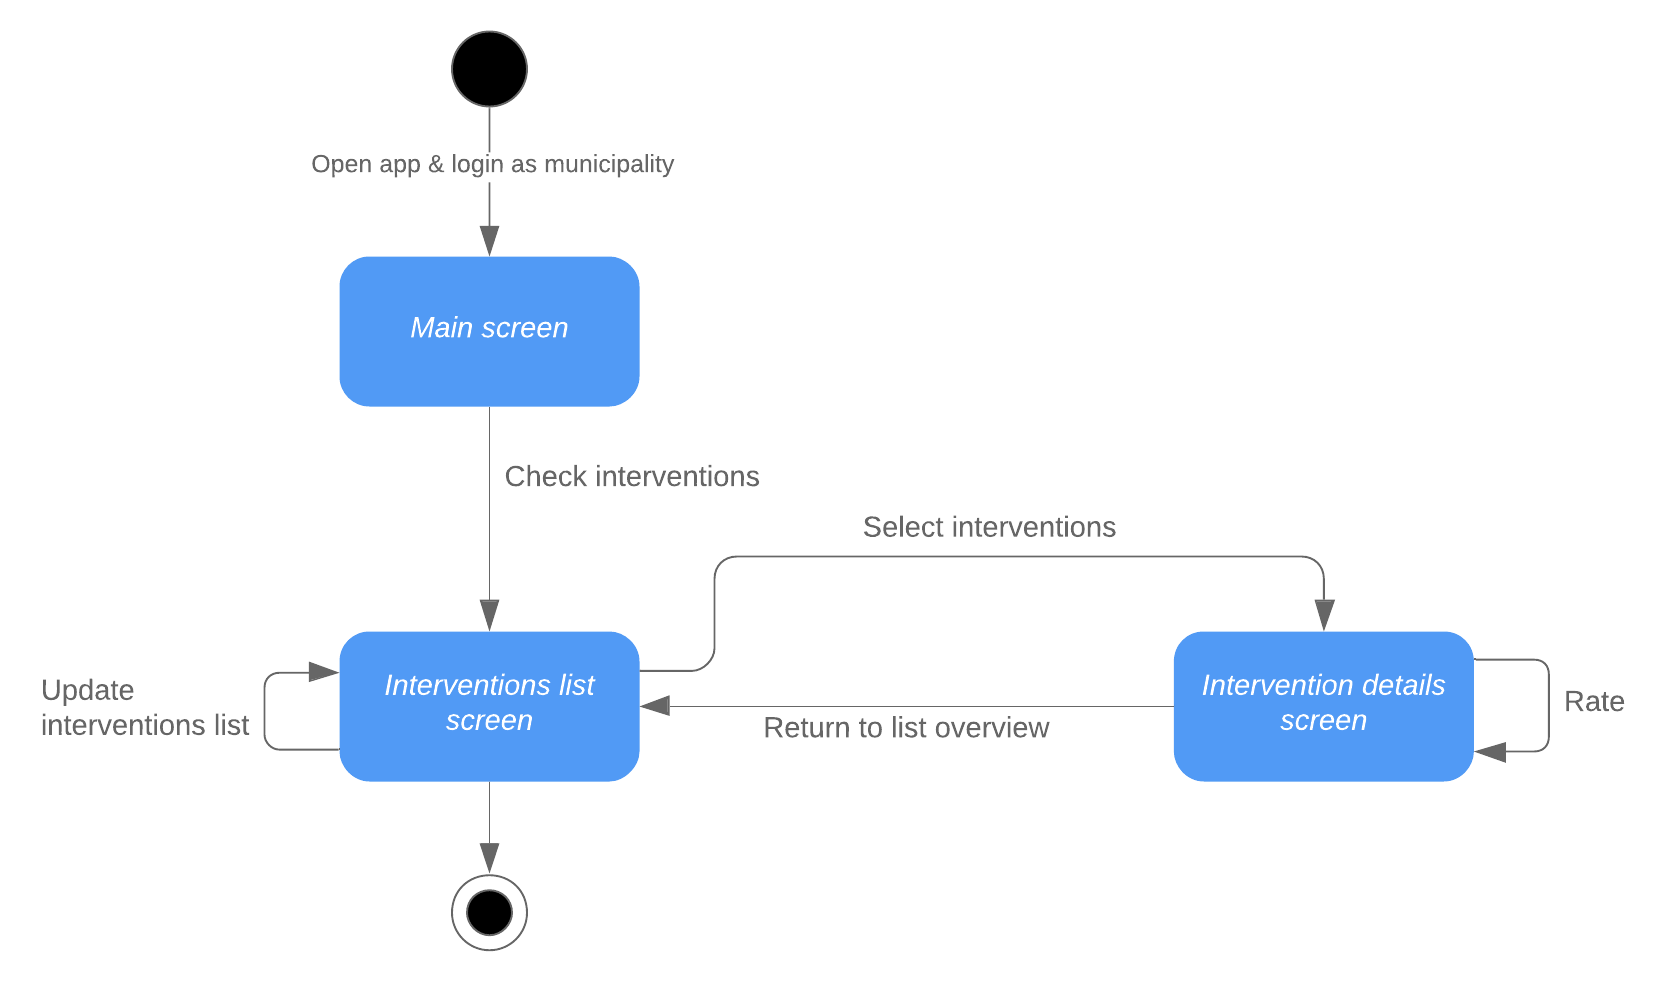
\includegraphics[width=\textwidth]{UML/SuggestionEvaluationStateDiagram}
	\caption{Suggestions evaluation state diagram}
\end{figure}

The flow of states that identifies the process of a municipality for checking the suggested interventions is pretty similar to the precedent. The municipalities can check, from the appropriate tab, a list of interventions relative to their city (updating it eventually) and then consult the interventions individually. They can also rate them to give a feedback to the system to improve future suggestions.

\subsubsection{Data analysis (any user)}

\begin{figure}[H]
	\centering
	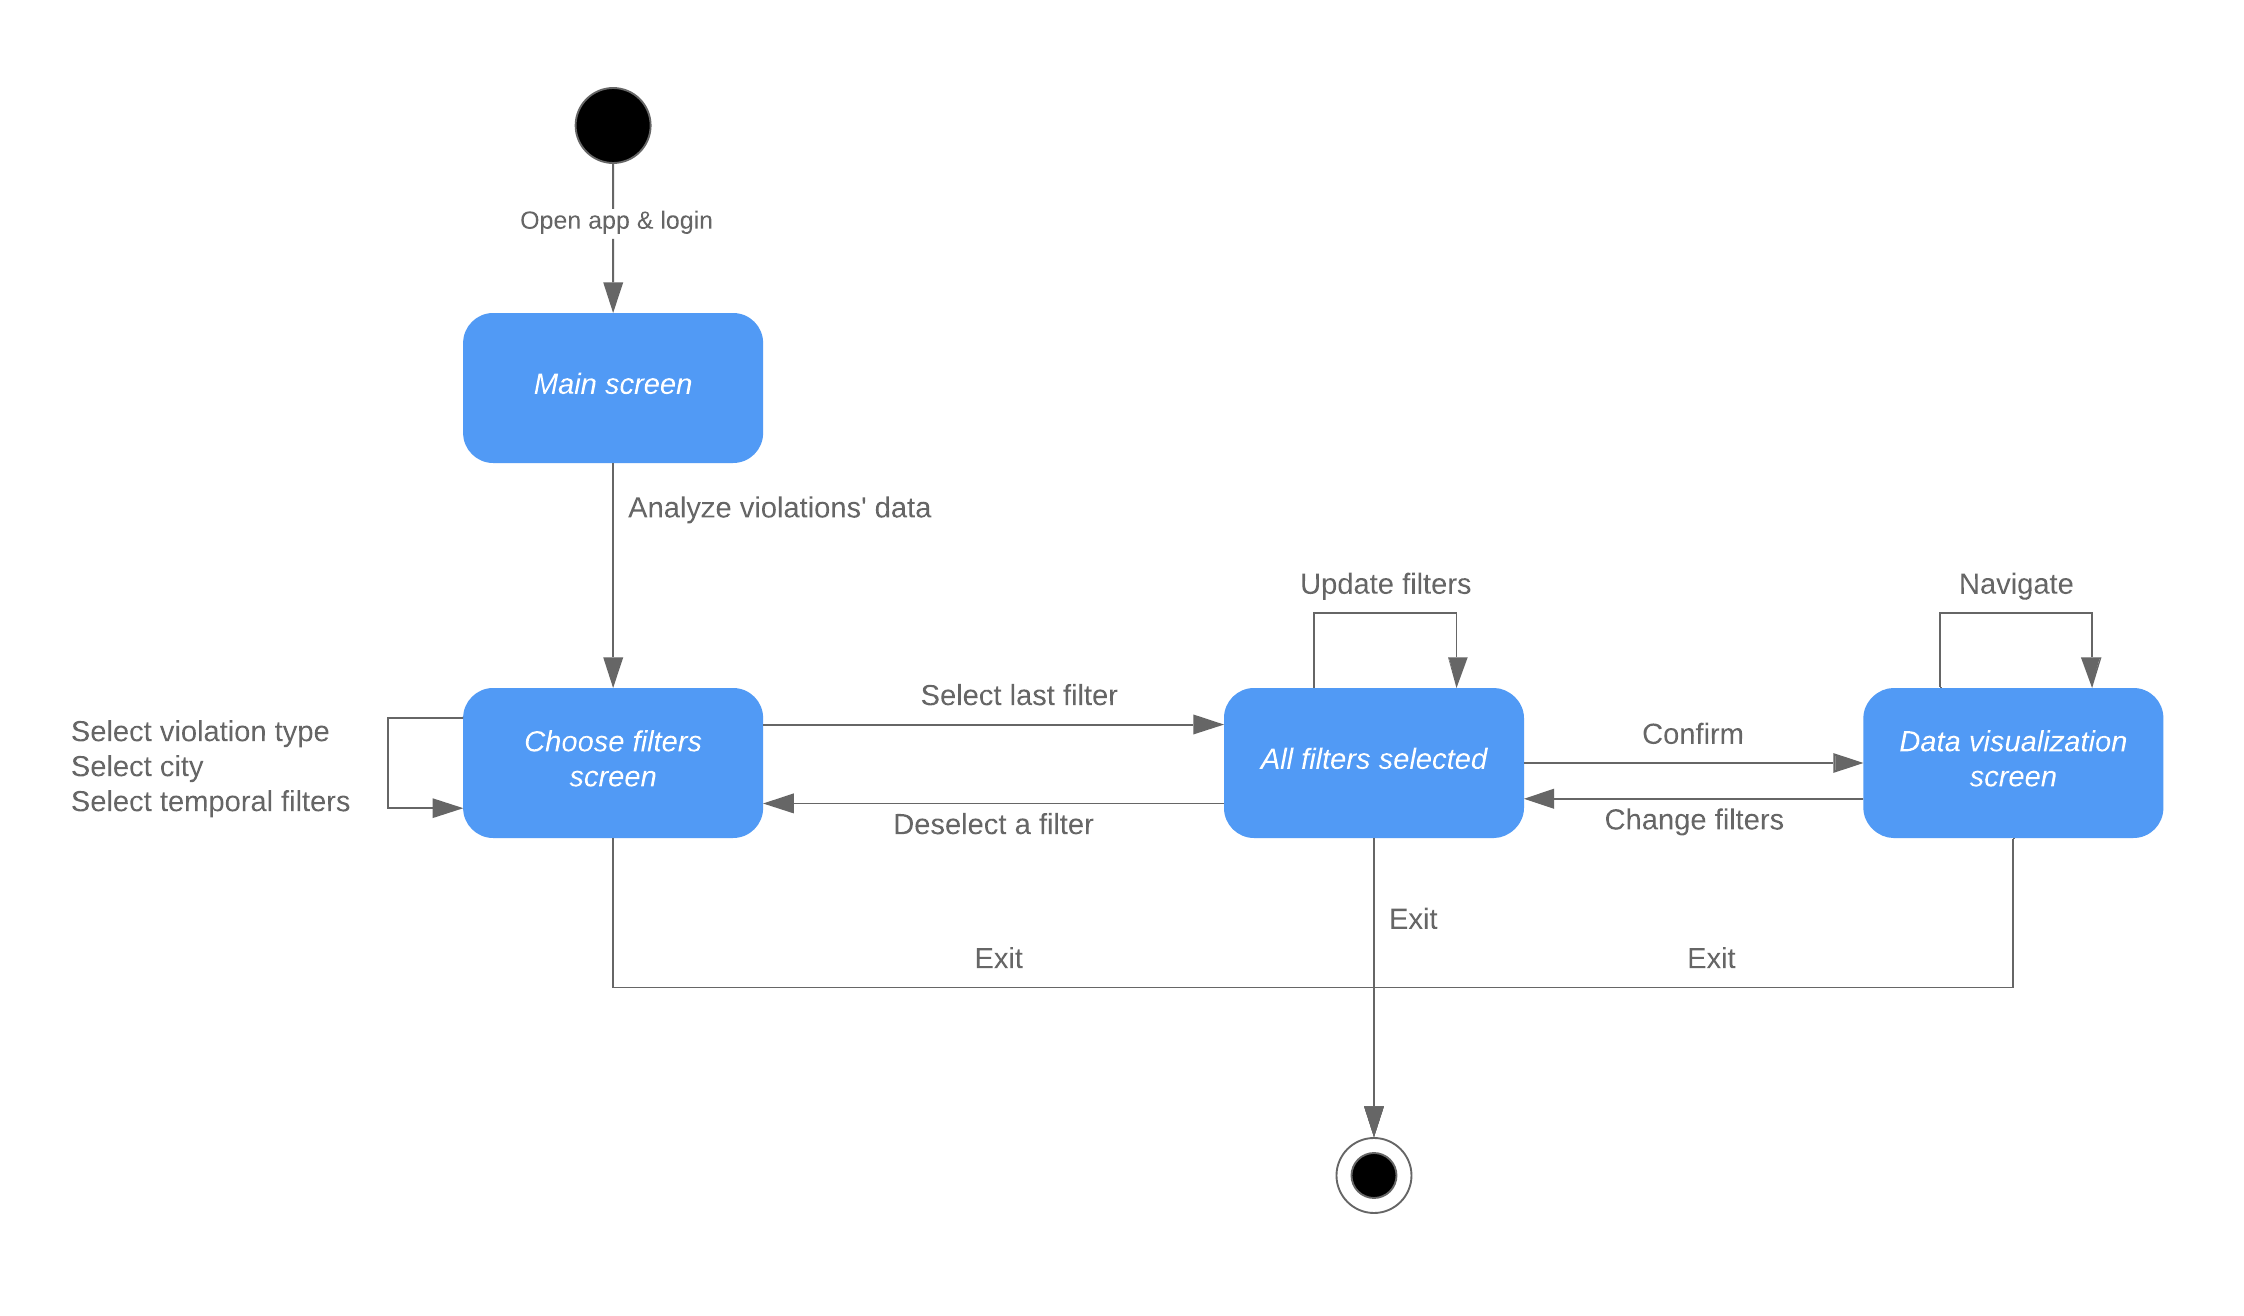
\includegraphics[width=\textwidth]{UML/AnalyzeDataStateDiagram}
	\caption{Data analysis state diagram}
\end{figure}

The final state diagram describes the process done by any type of user to analyze aggregate data of interest in a city map. In the appropriate tab, the user is asked to insert spatial and temporal filters, also specifying the type of violation (left to "all" value if not interested in a more specific research). Then the user can confirm to check a density map of the violations and a small report, containing auxiliary text data. At any time he can update the filters or end the operation.